\chapter{Prílohy}
\label{chap:prilohy}





\section{CD}
\label{chap:cd}


\begin{enumerate}[noitemsep,label*=\thesection.\arabic*.]
    \item diplomova\_praca
    
    \begin{enumerate}[noitemsep,label*=\arabic*.]
        \item praca
        
        \begin{enumerate}[noitemsep,label*=\arabic*.]
            \item praca.pdf
        \end{enumerate}
        
        \item zadanie\_diplomovej\_prace.pdf
    \end{enumerate}
    
    \item \label{item:prilohy_cd_eve_ng_adresar} eve\_ng
    
    \begin{enumerate}[noitemsep,label*=\arabic*.]
        \item profiling\_and\_benchmarking\_results
        
        \begin{enumerate}[noitemsep,label*=\arabic*.]
            \item 0\_pokojovy\_stav
            \item \label{item:all_benchmarks} adresáre s meraniami systémových požiadaviek pre každé zariadenie
        \end{enumerate}
        
        \item \label{item:skripty} skripty
        
        \begin{enumerate}[noitemsep,label*=\arabic*.]
            \item \label{item:uprava_sablon_skript} 10\_1\_update\_eve\_ng\_templates.sh
            \item \label{item:backup_script} 12\_1\_backup\_gns3\_and\_eveng\_data\_to\_backup\_server.sh
            \item \label{item:gns3_import_skript} import\_eveng\_qemu\_devices\_to\_gns3.sh
            \item CiscoIOUKeygen\_iougen\_eve-ng\_python2.py
            \item CiscoIOUKeygen\_iougen\_eve-ng\_python3.py
            \item CiscoIOUKeygen\_iougen\_gns3\_python2.py
            \item CiscoIOUKeygen\_iougen\_gns3\_python3.py
            \item dstat\_custom
        \end{enumerate}
        
        \item \label{item:vnc1} 01\_0\_vytvorenie\_vzdialenej\_pracovnej\_plochy\_nomachine.txt
        \item \label{item:vnc2} 01\_1\_vytvorenie\_vzdialenej\_pracovnej\_plochy\_vnc.txt
        \item \label{item:vnc3} 01\_2\_vytvorenie\_vzdialenej\_pracovnej\_plochy\_\_x2go\_BROKEN\_IN\_\\STRETCH
        \item \label{item:vmware_extra_instalacia} 02\_instalacia\_vmware\_player\_debian.txt
        \item 03\_hardverova\_konfiguracia\_EVE\_vo\_VMware\_Player.txt
        \item \label{item:instalacia_ubuntu_a_eve_ng} 04\_0\_instalacia\_eve\_ng.txt
        \item 04\_1\_instalacia\_eve\_ng\_do\_lxc\_kontajnera.txt
        \item \label{item:instalacia_A_konfiguracia_eve_ng} 05\_0\_prvotna\_konfiguracia\_EVE\_ng.txt
        \item \label{item:adresarova_struktura} 05\_1\_adresarova\_struktura\_uzitocne\_eve-ng\_subory.txt
        \item \label{item:zabezpecenie} 06\_zabezpecenie\_servera.txt
        \item 07\_0\_podporovane\_zariadenia\_v\_UNetLab\_EVE-ng.txt
        \item \label{item:pridavanie_konverzia_zariadeni} 07\_1\_pridavanie\_a\_konverzia\_zariadeni.txt
        \item 07\_2\_vypocet\_idle\_pc\_hodnot\_pre\_dynamips\_zariadenia.txt
        \item 07\_3\_pridanie\_cisco\_c2691\_do\_eve\_ng-CIASTOCNY\_USPECH.txt
        \item \label{item:pridavanie_juniper_vmx} 07\_4\_pridavanie\_zariadeni\_do\_eve\_ng\_juniper\_vmx\_17.3.txt
        \item 07\_5\_pridavanie\_zariadeni\_do\_eve\_ng\_cisco\_prime\_infra.txt
        \item 07\_6\_pridavanie\_zariadeni\_do\_eve\_ng\_vyos.txt
        \item 07\_7\_pridavanie\_zariadeni\_do\_eve\_ng\_pfsense.txt
        \item \label{item:pridavanie_cisco_asav} 07\_8\_pridavanie\_zariadeni\_do\_eve\_ng\_cisco\_asav.txt
        \item \label{item:pridavanie_win} 07\_9\_vytvorenie\_windows\_10\_kvm\_virtualky\_s\_virtio\_ovladacmi-\\CIASTOCNY\_USPECH.txt
        \item \label{item:iou_licencia} 08\_vytvorenie\_cisco\_iou\_iol\_licencie.txt
        \item 09\_0\_vytvorenie\_labu\_v\_eve\_ng.txt
        \item \label{item:uprava_sablon} 10\_0\_uprava\_sablon.txt
        \item \label{item:sprava_pouzivatelov_a_databazy} 11\_sprava\_pouzivatelov\_a\_MySQL\_databazy.txt
        \item \label{item:obnova_zalohovanie} 12\_0\_migracia\_zalohovanie\_obnovenie\_eve\_ng.txt
        \item \label{item:benchmarking_popis} 13\_0\_profiling\_and\_benchmarking.txt
        \item \label{item:benchmarking_list} 13\_1\_profiling\_and\_benchmarking\_device\_list.txt
        \item \label{item:aktualizacia_eve_ng} 14\_aktualizovanie\_eve\_ng.txt
        \item 15\_aktivacia\_podpory\_pre\_docker\_kontajnery-CIASTOCNY\_USPECH.txt
        \item \label{item:integracia_s_prehliadacmi} 16\_0\_eve-ng\_integracia\_s\_web\_prehliadacmi.txt
        \item 16\_1\_eve-ng\_odchytavanie\_prevadzky\_v\_topologii.txt
        \item \label{item:spristupnenie_pouzivatelskych_roli} 17\_00\_spristupnenie\_pouzivatelskych\_roli\_v\_EVE-ng\_web\_rozhrani.txt
        \item 17\_02\_eve\_ng-prihlasenie\_sa\_na\_server.pcapng
        \item 17\_03\_eve\_ng-vymazanie\_pouzivatela\_z\_web\_gui.pcapng
        \item 17\_04\_eve\_ng-vytvorenie\_pouzivatela\_z\_web\_gui.pcapng
        \item 17\_05\_eve\_ng-vytvorenie\_pouzivatela\_z\_web\_gui\_user\_role.pcapng
        \item 17\_06\_eve\_ng-prihlasenie\_pouzivatela\_time-8.606958977\\\_8.642465542.pcapng
        \item 17\_07\_eve\_ng-prihlasenie\_sa\_ako\_pouzivatel\_typu\_user\_time\\\_0.372278908.pcapng
        \item 17\_10\_eve\_ng-vypis\_vsetkych\_pouzivatelov\_z\_api\_FIX\_wireshark.pcapng
        \item \label{item:spristupnenie_pouzivatelskych_roli_pcap_posledny} 17\_11\_eve\_ng-vypis\_pouzivatela\_typu\_user\_z\_api\_wireshark.pcapng
        \item 18\_0\_eve\_ng-BUG-email\_a\_name\_ide\_nastavit\_ale\_nejde\_odstranit-time\\\_5.66\_18.198\_18.37-FollowHTTPStream\_136.025\_143.6.pcapng
        \item \label{item:mail_meno_nejde_odstranit} 18\_0\_eve\_ng-BUG-email\_a\_name\_ide\_nastavit\_ale\_nejde\_odstranit.txt
        \item \label{item:display_too_small} 19\_0\_eve\_ng-Display\_too\_small\_BUG.txt
        \item \label{item:nezobrazene_chybove_hlasenie} 20\_0\_eve\_ng-Nezobrazuje\_sa\_chybove\_hlasenie\_o\_nedostatocnych\\\_opravneniach\_pre\_BUG\_UNRESOLVED.txt
        \item \label{item:nezobrazene_chybove_hlasenie_pcap} 20\_2\_eve\_ng-Nezobrazuje\_sa\_chybove\_hlasenie\_o\_nedostatocnych\\\_opravneniach\_pre\_BUG\_UNRESOLVED.txt.pcapng
        \item \label{item:zatvorenie_topologie_so_spustenymi_zariadeniami} 21\_0\_eve\_ng-Topologia\_so\_spustenymi\_zariadeniami\_sa\_neda\_zatvorit.txt
        \item pripojenie\_unetlab\_eve\_ng\_k\_lokalnej\_sieti\_a\_internetu.odt
    \end{enumerate}
    
    \item materialy\_na\_predmety
    
    \begin{enumerate}[noitemsep,label*=\arabic*.]
        \item nasadenie\_do\_vyucovania
        
        \begin{enumerate}[noitemsep,label*=\arabic*.]
            \item Pocitacove\_siete\_2
            
            \begin{enumerate}[noitemsep,label*=\arabic*.]
                \item \label{item:nasadenie_ps2_benchmark} ps2\_7\_tyzden\_ppp\_topologia\_final\_8\_replik\_33\_IOL\_L3\_a\_16\\\_QEMU\_Alpine\_Linux.ods
                \item PS2\_7\_tyzden\_FINAL\_navrh.unl
                \item PS2\_7\_tyzden\_FINAL.unl
            \end{enumerate}
        \end{enumerate}
        
        \begin{enumerate}[noitemsep,label*=\arabic*.]
            \item Projektovanie\_sieti\_1
            
            \begin{enumerate}[noitemsep,label*=\arabic*.]
                \item PrS1\_9cv\_MPLS\_navrh.unl
                \item PrS1\_9cv\_MPLS\_set1.unl
                \item PrS1\_9cv\_MPLS\_set2.unl
            \end{enumerate}
        \end{enumerate}
        
        \begin{enumerate}[noitemsep,label*=\arabic*.]
            \item Projektovanie\_sieti\_2
            
            \begin{enumerate}[noitemsep,label*=\arabic*.]
                \item eVPN.unl
                \item Mcast VPN.unl
                \item Seamless MPLS.unl
                \item VPLS.unl
            \end{enumerate}
        \end{enumerate}
        
        \item \label{item:zoznam_technologii_s_podporou_zariadeni} 0\_0\_vyucovane\_technologie.ods
        \item \label{item:zoznam_technologii_txt} 0\_1\_zoznam\_technologii.txt
        \item \label{item:cisco_feature_testing_skript} 0\_2\_vyucovane\_technologie\_testovaci\_skript\_cisco.txt
    \end{enumerate}
    
    \item \label{item:sumarny_prehlad_zariadeni} sumarny\_prehlad\_podporovanych\_zariadeni\_vo\_virtualnych\_sietovych\\\_nastrojoch.ods
    \item \label{item:zdroje_informacii_a_zariadeni} zdroje\_informacii\_a\_zariadeni.txt
    \item \label{item:monitorovanie} monitorovanie\_servera\_netdata.txt
    \item \label{item:upraveny_integracny_balicek_linux} eve-ng-integration\_kis
\end{enumerate}





\newpage

\section{Používanie EVE-ng}
\label{chap:pouzivanie_eve_ng}

V tejto kapitole opisujem kroky na vytvorenie topológie následnú prácu so zariadeniami v nej v nástroji EVE-ng.




\subsection{Vytvorenie topológie}
\label{chap:vytvorenie_topo_eve-ng}
Topológie sa vytvárajú prostredníctvom webového rozhrania EVE-ng. Nižšie sú uvedené kroky na vytvorenie topológie v EVE-ng.

\begin{enumerate}[noitemsep]

    \item \label{item:prihlasenie} Najprv sa prihlásime do nástroja EVE-ng cez webové rozhranie v natívnom móde - \emph{Native console} (obr. \ref{obr:eve_ng_login_screen}). Webové rozhranie je dostupné v 2 módoch: natívnom a HTML5. Rozdiely medzi jednotlivými módmi sú popísané v bode \ref{item:vzdialeny_pristup}. Pre úspešné prihlásenie musíme mať vytvorený používateľský účet, čo môže urobiť iba používateľ s rolou \emph{admin}.

\begin{figure}
    \centering
    \includegraphics[width=0.6\textwidth,trim={15cm 0cm 15cm 4cm},clip]{eve_ng_login_screen}
    \caption{Prihlasovacia obrazovka EVE-ng}
    \label{obr:eve_ng_login_screen}
\end{figure}

    \item Po prihlásení sa zobrazí hlavná obrazovka (obr. \ref{obr:eve_ng_main_screen}). V ľavej časti sa nachádza správca súborov, v ktorom si vyberieme adresár, kde bude uložený súbor s topológiou.

\begin{figure}
    \centering
    \includegraphics[width=1\textwidth,trim={0cm 0cm 0cm 4cm},clip]{eve_ng_main_screen}
    \caption{Hlavná obrazovka EVE-ng}
    \label{obr:eve_ng_main_screen}
\end{figure}

    \item Po výbere adresára klikneme na ikonku hárku s popisom \emph{Add new lab} (obr. \ref{obr:eve_ng_lab_menu}), čím začneme vytváranie novej topológie. Topológiu môže vytvoriť iba používateľ s rolou \emph{editor} alebo \emph{admin}.

\begin{figure}
    \centering
        \includegraphics[width=0.75\textwidth,trim={1.2cm 14.6cm 32cm 8.5cm},clip]{eve_ng_lab_menu}
    \caption{Menu pre úpravu súborov}
    \label{obr:eve_ng_lab_menu}
\end{figure}

    \item Zobrazí sa dialógové okno, do ktorého zadáme atribúty topológie (obr. \ref{obr:eve_ng_lab_dialog}). Pre úspešné vytvorenie súboru stačí vyplniť iba povinné atribúty: \emph{Name} (názov topológie) a \emph{Version} (verzia topológie).

\begin{figure}
    \centering
    \includegraphics[width=1\textwidth,trim={1.7cm 4.8cm 1.7cm 7.5cm},clip]{eve_ng_lab_dialog}
    \caption{Dialógové okno na vytvorenie nového súboru s topológiou}
    \label{obr:eve_ng_lab_dialog}
\end{figure}

    \item Po kliknutí na tlačidlo \emph{Save} sa súbor s topológiou vytvorí a následne sa zobrazí pracovná plocha na vytvorenie topológie (obr. \ref{obr:eve_ng_nova_topologia}). Novovytvorená topológia je prázdna.

\begin{figure}
    \centering
    \includegraphics[width=0.75\textwidth,trim={0cm 4cm 20cm 4cm},clip]{eve_ng_nova_topologia}
    \caption{Ukážka novovytvorenej (prázdnej) topológie s ovládacím panelom}
    \label{obr:eve_ng_nova_topologia}
\end{figure}

    \item Do topológie môžeme po jej vytvorení pridávať tieto prvky:
    
    \begin{description}[noitemsep]
        \item [Node] zariadenie
        \item [Network] sieť
        \item [Picture] obrázok
        \item [Custom Shape] geometrický tvar - obdĺžnik/elipsa
        \item [Text] textové polia
    \end{description}
    
    Spomenutý zoznam prvkov (obr. \ref{obr:eve_ng_add_new_object_context_menu}) sa zobrazí v kontextovom menu po pravom kliknutí na prázdne miesto v topológii alebo po kliknutí na ikonku \textbf{+} v menu na ľavej strane obrazovky.
    
\begin{figure}
    \centering
    \includegraphics[width=0.2\textwidth,trim={0cm 0cm 0cm 0.1cm},clip]{eve_ng_add_new_object_context_menu}
    \caption{Kontextové menu pre pridanie zariadenia}
    \label{obr:eve_ng_add_new_object_context_menu}
\end{figure}
    
    Keď chceme pridať do topológie napríklad zariadenie, v kontextovom menu klikneme na možnosť \emph{Node}. Následne sa zobrazí dialógové okno pre vyhľadanie zariadenia (obr. \ref{obr:eve_ng_add_a_new_node_selection_dialog}). Vyhľadávanie si môžeme uľahčiť tak, že do vyhľadávacieho riadku napíšeme úvodné znaky pridávaného modelu zariadenia. Po jeho výbere sa zobrazí dialógové okno na úpravu jeho parametrov (obr. \ref{obr:eve_ng_add_a_new_node_3725_edit_dialog}). Jediné polia, ktorými by sa používateľ potreboval zaoberať, sú \emph{Name/prefix} (názov zariadenia) a \emph{Number of nodes to add} (počet zariadení, ktoré sa do topológie pridajú naraz). Všetky ostatné polia sú už nastavené a nie je potrebné ich meniť.
    
    Po kliknutí na tlačidlo \emph{Save} sa do topológie pridá toľko zariadení, koľko bolo zadaných do poľa \emph{Number of nodes to add}. Pre každé zariadenie sa vygeneruje a priradí portové číslo, pomocou ktorého bude možné, pripojiť sa na jeho konzolu. Generovanie portových čísel pre zariadenia v EVE-ng je bližšie vysvetlené v časti \ref{chap:priradovanie_portovych_cisel} - \nameref{chap:priradovanie_portovych_cisel}.
    
\begin{figure}
    \centering
    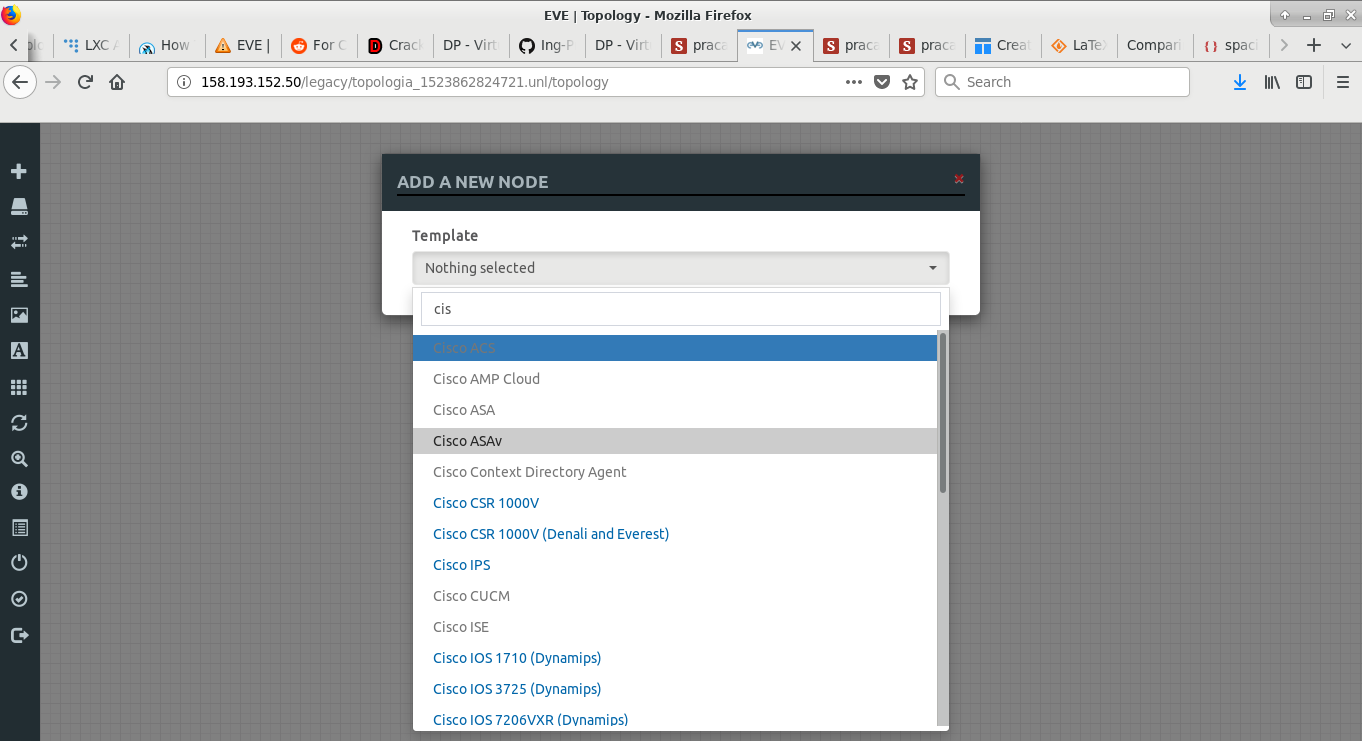
\includegraphics[width=0.65\textwidth,trim={12cm 0cm 12cm 5cm},clip]{eve_ng_add_a_new_node_selection_dialog}
    \caption{Dialógové okno pre vyhľadanie zariadenia}
    \label{obr:eve_ng_add_a_new_node_selection_dialog}
    
    \vspace{1cm}
    
    \centering
    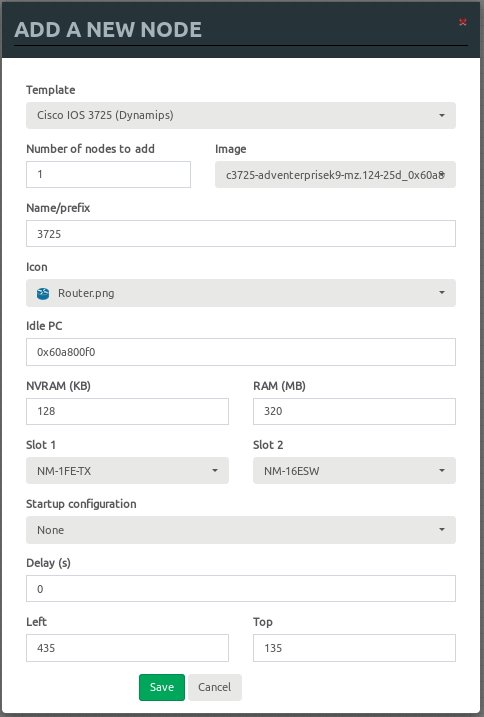
\includegraphics[width=0.5\textwidth,trim={0cm 0.1cm 0.1cm 0.1cm},clip]{eve_ng_add_a_new_node_3725_edit_dialog}
    \caption{Dialógové pre úpravu parametrov pridávaného zariadenia}
    \label{obr:eve_ng_add_a_new_node_3725_edit_dialog}
\end{figure}
    
    \item Po pridaní prvkov do topológie vytvoríme spojenia medzi jednotlivými zariadeniami. Zariadenia je možné prepájať iba rozhraniami rovnakého typu (Ethernet-Ethernet, Serial-Serial). Prepájať je možné iba \emph{vypnuté} zariadenia. Prepojenie medzi zariadeniami vytvoríme kliknutím na ikonu \emph{vidlice} s popisom \emph{Connect to another node} (obr. \ref{obr:eve_ng_prepajanie_vidlica}) a potiahnutím myši smerom ku druhému zariadeniu (obr. \ref{obr:eve_ng_prepajanie_ku_druhemu_zariadeniu}). Následne sa objaví dialógové okno s výberom rozhraní pre obidve zariadenia, ktoré majú byť prepojené (obr. \ref{obr:eve_ng_prepajanie_add_connection_dialog}). Po výbere rozhraní z oboch rozbaľovacích zoznamov klikneme na tlačidlo \emph{Save}. Dialógové okno sa zatvorí a vytvorí sa prepojenie medzi zariadeniami pre zvolené rozhrania (obr. \ref{obr:eve_ng_prepajanie_prepojenie_vytvorenie}). Po nastavení správnych IP adries na prepojených rozhraniach bude vytvorená konektivita medzi zariadeniami.
    
    \begin{comment}
    \begin{figure}
        \centering
        \includegraphics[width=0.5\textwidth,trim={8cm 15cm 30cm 7cm},clip]{eve_ng_prepajanie_vidlica}
        \caption{Ikona na prepájanie zariadení}
        \label{obr:eve_ng_prepajanie_vidlica}
        
        \centering
        \includegraphics[width=0.5\textwidth,trim={8cm 15cm 30cm 7cm},clip]{eve_ng_prepajanie_ku_druhemu_zariadeniu}
        \caption{Priebeh prepájania zariadení}
        \label{obr:eve_ng_prepajanie_ku_druhemu_zariadeniu}
    \end{figure}
    \end{comment}
    
    
    \begin{figure}
    %\centering
    \begin{minipage}{.5\textwidth}
        \centering
        \includegraphics[width=0.9\textwidth,trim={8cm 15cm 30cm 7cm},clip]{eve_ng_prepajanie_vidlica}
        \caption{Ikona na prepájanie zariadení}
        \label{obr:eve_ng_prepajanie_vidlica}
    \end{minipage}%
    \begin{minipage}{.5\textwidth}
        \centering
        \includegraphics[width=0.9\textwidth,trim={8cm 15cm 30cm 7cm},clip]{eve_ng_prepajanie_ku_druhemu_zariadeniu}
        \caption{Priebeh prepájania zariadení}
        \label{obr:eve_ng_prepajanie_ku_druhemu_zariadeniu}
    \end{minipage}
    \end{figure}
    
    
    
    
    
    \begin{figure}
        \centering
        \includegraphics[width=0.75\textwidth]{eve_ng_prepajanie_add_connection_dialog}
        \caption{Dialógové okno na výber prepájaných rozhraní}
        \label{obr:eve_ng_prepajanie_add_connection_dialog}
    \end{figure}
    
    \begin{figure}
        \centering
        \includegraphics[width=0.5\textwidth,trim={8cm 15cm 30cm 7cm},clip]{eve_ng_prepajanie_prepojenie_vytvorenie}
        \caption{Úspešné vytvorenie prepojenia}
        \label{obr:eve_ng_prepajanie_prepojenie_vytvorenie}
    \end{figure}
    
    \item Po prepojení prvkov v topológii je možné upravovať ich atribúty rôznymi spôsobmi.
    
    \begin{itemize}[noitemsep]
        \item Najjednoduchším spôsobom úpravy platným pre všetky prvky je presunutie prvku myšou.
        \item Zariadenia je možné upravovať v zozname zariadení po kliknutí na položku \emph{Nodes} v menu na ľavej strane obrazovky (obr. \ref{obr:eve_ng_configured_nodes_dialog}).
        \item Ďalší spôsob, ako upraviť parametre zariadenia je pravým kliknutím na zariadenie a kliknutím na \emph{Edit} (obr. \ref{obr:eve_ng_edit_node_dialog}).
        \item Siete sa dajú upravovať v zozname sietí po kliknutí na položku \emph{Networks} v menu na ľavej strane obrazovky (obr. \ref{obr:eve_ng_configured_networks_dialog}).
        \item Obrázky, geometrické tvary a textové polia vieme upravovať v zozname objektov po kliknutí na položku \emph{Configured objects} v menu na ľavej strane obrazovky (obr. \ref{obr:eve_ng_configured_objects_dialog}).
    \end{itemize}

\begin{figure}
    \centering
    \includegraphics[width=1\textwidth,trim={2cm 13cm 2cm 5cm},clip]{eve_ng_configured_nodes_dialog}
    \caption{Dialógové okno so zoznamom zariadení v topológii}
    \label{obr:eve_ng_configured_nodes_dialog}
\end{figure}

\begin{figure}
    \centering
    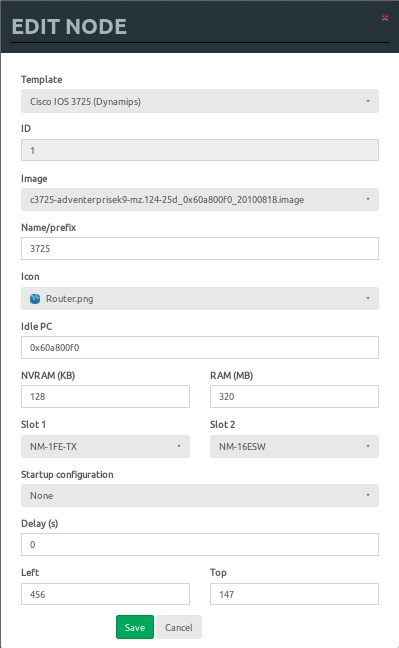
\includegraphics[width=0.6\textwidth,trim={0.1cm 0cm 0cm 0cm},clip]{eve_ng_edit_node_3725_edit_dialog}
    \caption{Dialógové okno na úpravu zariadenia}
    \label{obr:eve_ng_edit_node_dialog}
\end{figure}

\begin{figure}
    \centering
    \includegraphics[width=1\textwidth,trim={2cm 13cm 2cm 5cm},clip]{eve_ng_configured_networks_dialog}
    \caption{Dialógové okno so zoznamom sietí v topológii}
    \label{obr:eve_ng_configured_networks_dialog}
\end{figure}

\begin{figure}
    \centering
    \includegraphics[width=1\textwidth,trim={2cm 13cm 2cm 5cm},clip]{eve_ng_configured_objects_dialog}
    \caption{Dialógové okno so zoznamom grafických a textových objektov}
    \label{obr:eve_ng_configured_objects_dialog}
\end{figure}



    
Ďalší spôsob na úpravu prvkov v topológii je upravovanie samotného súboru s topológiou na serveri s príponou \emph{unl} (obr. \ref{obr:eve_ng_unl_file_syntax}). Tieto súbory sú napísané vo formáte XML a sú uložené v adresári \texttt{/opt/unetlab/labs/}. Súbory môže upravovať iba administrátor EVE-ng servera alebo používatelia so \emph{sudo} oprávneniami. Prvky sú definované značkami, ktoré definujú ich typ (zariadenie, sieť, textové pole a pod.). Nižšie je uvedený zoznam niektorých značiek použitých v \emph{unl} súbore.

    \begin{description}[noitemsep]
        \item [\texttt{<node>}] - zariadenie v topológii
        \begin{description}[noitemsep]
            \item [\texttt{id}] - identifikačné číslo zariadenia; slúži na vygenerovanie portového čísla; musí byť unikátne
            \item [\texttt{name}] - názov zariadenia; zobrazuje sa pod jeho ikonkou; malo by byť unikátne, kvôli prehľadnosti topológie
            \item [\texttt{left}] - vzdialenosť od ľavého okraja plochy v topológii
            \item [\texttt{top}] - vzdialenosť od horného okraja plochy v topológii
            \item [\texttt{uuid}] - UUID identifikátor zariadenia; musí byť unikátny; iba pre QEMU zariadenia
            \item [\texttt{firstmac}] - MAC adresa prvého rohzrania pre zariadenia; iba pre QEMU zariadenia
            \item [\texttt{<interface>}] - pripojené rozhrania pre zariadenie
            \begin{description}[noitemsep]
                \item [\texttt{id}] - identifikačné číslo pripojeného rozhrania; musí byť unikátne
                \item [\texttt{remote\_id}] - identifikačné číslo vzdialeného zariadenia - odkaz na atribúť \texttt{id} v značke \texttt{<node>} iného zariadenia; iba pre zariadenia typu IOL
                \item [\texttt{network\_id}] - identifikačné číslo siete; iba pre Ethernet rozhrania 
            \end{description}
        \end{description}
        
        \item [\texttt{<networks>}] - zoznam vytvorených sietí v topológii
        \begin{description}[noitemsep]
            \item [\texttt{<network>}] - sieť v topológii; vytvára sa ako \emph{bridge} rozhranie pre prepojenie dvoch Ethernet rozhraní medzi zariadeniami alebo pri pridaní siete z kontextového menu pri zvolení položky \emph{Network}
            \begin{description}[noitemsep]
                \item [\texttt{id}] - identifikačné číslo siete; musí byť unikátne
                \item [\texttt{visibility}] - viditeľnosť siete; v prípade, že prepájame dve Ethernet rohrania, je atribút nastavený na hodnotu 0 - sieť (bridge rozhranie) je v topológii skrytá; ak pridávame do topológie sieť explicitne cez \emph{Add a new object} -> \emph{Network}, atribút sa nastaví na hodnotu 1 a sieť bude viditeľná v topológii
            \end{description}
        \end{description}
    \end{description}

Zmeny v \emph{unl} súbore sa prejavia až po znovunačítaní stránky (klávesou F5) alebo topológie (kliknutím na \emph{Refresh topology} v menu na ľavej strane obrazovky).

\begin{figure}
    \centering
    \includegraphics[width=0.75\textwidth,trim={0cm 0cm 0cm 1.9cm},clip]{eve_ng_unl_file_syntax}
    \caption{Ukážka UNL súboru}
    \label{obr:eve_ng_unl_file_syntax}
\end{figure}
    
Experimentovaním sme zistili, že vytváranie topológii a duplikácia jej prvkov v \emph{unl} súbore je pomerne náročná, zdĺhavá a náchylná na chyby. Pri duplikácii zariadení bolo náročné udržať prehľad o.i. aj o identifikátoroch zariadení a rozhraní a ich vzájomnom prepojení. Výhodnejšie sa ukázalo najprv použiť webové rozhranie, potom tabuľku zariadení \emph{Nodes} a nakoniec upraviť \emph{unl} súbor:
    
    \begin{enumerate}[noitemsep]
        \item Najpr vo webovom rozhraní vytvoríme topológiu, pridáme do nej zariadenia a poprepájame ich.
        \item Potom v tabuľke zariadení \emph{Nodes} upravíme názvy zariadení v stĺpci \emph{Name} (obr. \ref{obr:eve_ng_configured_nodes_dialog}).
        \item Ak je potrebné, nakoniec v \emph{unl} súbore presnejšie upravíme súradnice prvkov v topológii definovaných atribútmi \texttt{left} a \texttt{top}. Výsledkom týchto úprav je celkové zlepšenie vzhľadu topológie. Môžeme tak urobiť aj vo webovom rozhraní v dialógovom okne pre úpravu zariadenia v atribútoch \emph{Left} a \emph{Top}, avšak v \emph{unl} súbore vieme súradnice prvkov upraviť hromadne.
    \end{enumerate}
    
    \item Potom, ako sme pridali zariadenia do topológie a navzájom ich prepojili, ich môžeme spustiť. Zariadenia sa dajú spustiť buď jednotlivo, skupinovo alebo všetky naraz. Zariadenia môže spúšťať iba používateľ s rolou \emph{admin} alebo \emph{editor}.

    \begin{itemize}[noitemsep]
        \item Jedno zariadenie spustíme tak, že naň klikneme pravým tlačidlom a zvolíme \emph{Start} (obr. \ref{obr:eve_ng_spustanie_po_jednom_context_menu}).
        \item Skupinu zariadení spustíme tak, že ich najpr označíme myšou resp. vyberieme zariadenia kombináciou \emph{Ctrl + ľavé kliknutie}. Následne na jedno z označených zariadení klikneme pravým tlačidlom a zvolíme \emph{Start Selected} (obr. \ref{obr:eve_ng_spustanie_skupiny_context_menu}).
        \item Všetky zariadenia spustíme kliknutím na položku \emph{More actions} a zvolíme možnosť \emph{Start all nodes} (obr. \ref{obr:eve_ng_spustanie_vsetkych_context_menu}).
    \end{itemize}

\begin{comment}
\begin{figure}
    \centering
    \includegraphics[width=0.3\textwidth,trim={11cm 5cm 28cm 9cm},clip]{eve_ng_spustanie_po_jednom_context_menu}
    \caption{Spustenie jedného zariadenia}
    \label{obr:eve_ng_spustanie_po_jednom_context_menu}
\end{figure}

\begin{figure}
    \centering
    \includegraphics[width=0.4\textwidth,trim={11cm 3cm 19cm 9cm},clip]{eve_ng_spustanie_skupiny_context_menu}
    \caption{Spustenie skupiny zariadení}
    \label{obr:eve_ng_spustanie_skupiny_context_menu}
\end{figure}
\end{comment}

\begin{figure}
%\centering
\begin{minipage}{.4\textwidth}
    \vspace{1.1cm}
    \centering
    \includegraphics[width=0.8\textwidth,trim={11cm 5cm 27cm 9cm},clip]{eve_ng_spustanie_po_jednom_context_menu}
    \caption{Spustenie jedného zariadenia}
\label{obr:eve_ng_spustanie_po_jednom_context_menu}
\end{minipage}%
\begin{minipage}{.6\textwidth}
    \centering
    \includegraphics[width=1\textwidth,trim={11cm 3cm 19cm 9cm},clip]{eve_ng_spustanie_skupiny_context_menu}
    \caption{Spustenie skupiny zariadení}
    \label{obr:eve_ng_spustanie_skupiny_context_menu}
\end{minipage}
\end{figure}

\begin{figure}
    \centering
    \includegraphics[width=0.6\textwidth,trim={0cm 3cm 29cm 9cm},clip]{eve_ng_spustanie_vsetkych_sidemenu}
    \caption{Spustenie všetkých zariadení}
    \label{obr:eve_ng_spustanie_vsetkych_context_menu}
\end{figure}
      
    \item \label{item:vzdialeny_pristup} Po spustení zariadení sa sprístupní ich vzdialená konzola. Spôsob, akým sa na pripájame na konzoly zariadení sa líši podľa toho, v akom móde sme sa do EVE-ng prihlásili. V bode \ref{item:prihlasenie} sme spomenuli, že do webového rozhrania EVE-ng sa dá prihlásiť v dvoch režimoch: v HTML5 alebo natívnom móde. Výber módu priamo ovplyvňuje aj spôsob, akým pristupujeme ku konzolám zariadení.
    
    HTML5 mód zabezpečuje vzdialený prístup k zariadeniam pomocou reverzného proxy servera \emph{Apache Guacamole}, ktorý sa pripája na konzoly zariadení. V tomto móde sa na obrazovke s otvorenou topológiou po kliknutí na zariadenie otvorí jeho vzdialená konzola, pričom nie je možné pripojiť sa ku konzolám zariadenia pomocou telnet alebo vnc klienta. HTML5 mód web rozhrania EVE-ng bol však menej stabilný a reagoval výrazne pomalšie pri práci s topológiou v provonaní s natívnym módom. Preto bolo webové rozhranie ďalej používané iba v natívnom režime.
        
    Natívny režim vyžaduje, aby sme mali pre vzdialený prístup ku zariadeniam na lokálnom počítači nainštalované dodatočné nástroje. 
        
    Na prístup k zariadeniam z lokálneho počítača potrebujeme mať nainštalovaného telnet a VNC klienta. Pre platformu Windows môžeme zvoliť kombináciu napr. \emph{PuTTY} a \emph{RealVNC Viewer}, pre platformu Linux zase terminál, napr. \emph{BASH} a \emph{TigerVNC}. Následne sa navigujeme myšou na zariadenie, na ktoré sa chceme pripojiť, ale namiesto toho, aby sme naň klikli, zapamätáme si údaje zobrazené v ľavom alebo pravom dolnom rohu obrazovky (obr. \ref{obr:eve_ng_protokol_ip_port}) t.j. protokol, IP adresa servera a portové číslo. Tieto údaje následne zadáme do zodpovedajúceho klienta podľa protokolu. Po zadaní správnych údajov by sme sa mali pripojiť na vzdialenú konzolu zariadenia.

\begin{figure}
    \centering
    \includegraphics[width=0.6\textwidth,trim={0cm 0cm 0.8cm 4cm},clip]{eve_ng_protokol_ip_port}
    \caption{Adresa na vzdialený prístup k zariadeniu (vľavo dole)}
    \label{obr:eve_ng_protokol_ip_port}
\end{figure}

    Aby sme mohli pristupovať ku konzole zariadenia z webového rozhrania pri kliknutí naň, potrebujeme mať na lokálnom počítači nainštalovaný tzv. EVE-ng integračný balíček. Ten existuje pre platformy Windows a Linux. Ďalej sme upravovali iba integračný balíček pre platformu Linux, z ktorého nakoniec vznikla ďalšia, bezpečnejšia verzia. Jednalo sa úpravy, ktoré zabezpečovali vzdialený prístup k zariadeniam s protokolmi \emph{telnet} a \emph{vnc} pomocou SSH tunelov a odchytávanie prevádzky z rozhrania zariadenia ako štandardný používateľ namiesto používateľa \emph{root}. Predvolený integračný baliček takéto funkciu neobsahuje. Vykonané úpravy nemajú výrazný vplyv na funkcionalitu pre koncového používateľa.
    
    Predvolené verzie integračných balíčkov je možné stiahnuť zo zdroja \cite{eve_ng_integration_pack_win} pre platformu Windows a zo zdroja \cite{eve_ng_integration_pack_linux} pre platformu Linux. Inštalácia a popis jednotlivých úprav integračného balíčka EVE-ng pre platformy Windows a Linux je popísaná v kapitole \ref{chap:cd} v bode \ref{item:integracia_s_prehliadacmi} Upravená verzia integračného balíčka pre platformu Linux je dostupná v kapitole \ref{chap:cd} v bode \ref{item:upraveny_integracny_balicek_linux}

\end{enumerate}

Vyššie uvedené kroky popisujú vytvorenie základnej topológie s rôznymi prvkami. V ďalších častiach bude popísané, ako EVE-ng generuje a priďeľuje portové čísla zariadeniam, pomocou ktorých sa pripájame na ich vzdialené konzoly a to, ako prepojiť viacero topológii medzi sebou resp. ako pripojiť topológiu k internetu.




\subsection{Prideľovanie portových čísel zariadeniam}
\label{chap:priradovanie_portovych_cisel}

Po pridaní ľubovoľného zariadenia do topológie sa preň vygeneruje portové číslo, ktoré mu je následne priradené. Portové čísla rozlišujú zariadenia v topológii a  slúžia na pripojenie sa na ich vzdialené konzoly. Vždy sa vyberie najnižšie dostupné portové číslo.

Rozsah portových čísel pre daného používateľa sa generujú vzťahom \emph{32768 + 128 * POD + ID}, kde \emph{POD} je unikátne identifikačné číslo používateľa a \emph{ID} je unikátne identifikačné číslo zariadenia. Za uvedený výpočet je zodpovená funkcia \texttt{\_\_construct} v súbore \\ \emph{/opt/unetlab/html/includes/\_\_node.php}.

Ak do topológie pridáme viacero zariadení naraz, budú mať portové čísla idúce za sebou.

V prípade, že si rôzni používatelia otvoria rovnaký súbor s topológiou, bude mať každý z používateľov prístup ku vlastným zariadeniam. Pokiaľ bude počet zariadení v topológii <= 63, portové čísla zariadení sa nebudú prekrývať a každý z používateľov bude môcť pracovať s topológiou nezávisle na sebe. Ak ľubovoľný z používateľov do topológie pridá zariadenie, uvidia ho všetci, ale až po obnovení topológie (F5/\emph{Refresh topology}).

Vyššie uvedené správanie bolo otestované po otvorení rovnakého súboru s topológiou dvomi rôznymi používateľmi s rôznymi používateľskými rolami (\emph{admin} a \emph{editor}).

S prideľovaním portových čísel súvisí aj problém popísaný v časti \ref{chap:zatvorenie_topo_so_spustenymi_zariadeniami}, pretože do vzťahu na výpočet portového čísla sa neberie do úvahy počet topológii, ktoré má používateľ spustené.

%Na obr. \ref{obr:eve_ng_rovnaka_topo_prvy_pouzivatel_admin} vidíme, že prvý používateľ už má spustené zariadenia, ale druhý používateľ ich ako spustené nevidí (obr. \ref{obr:eve_ng_rovnaka_topo_druhy_pouzivatel_editor}).

\begin{comment}
\begin{figure}
    \centering
    \includegraphics[width=0.75\textwidth,trim={0cm 0cm 0cm 4cm},clip]{eve_ng_rovnaka_topo_prvy_pouzivatel_admin}
    \caption{Topológia prvého používateľa s používateľskou rolou \emph{admin}}
    \label{obr:eve_ng_rovnaka_topo_prvy_pouzivatel_admin}
\end{figure}

\begin{figure}
    \centering
    \includegraphics[width=0.75\textwidth,trim={0cm 0cm 0cm 4cm},clip]{eve_ng_rovnaka_topo_druhy_pouzivatel_editor}
    \caption{Topológia druhého používateľa s používateľskou rolou \emph{editor}}
    \label{obr:eve_ng_rovnaka_topo_druhy_pouzivatel_editor}
\end{figure}
\end{comment}



\subsection{Pripojenie topológie k internetu / prepojenie topológii navzájom}

Do EVE-ng topológie je možné pridať prvok typu \emph{sieť}, ktorý umožňuje prepájať topológie medzi sebou alebo ich pripájať ku internetu.

Sieť do topológie pridáme kliknutím na ikonu \textbf{+} (\emph{Add an object}) a zo zoznamu vybierieme položku \emph{Network}. Objaví sa dialógové okno na úpravu parametrov pridávanej siete (obr. \ref{obr:eve_ng_add_network_dialog}). Pre správnu funkčnosť a prehľadnosť stačí zmeniť iba atribúty \emph{Name} a \emph{Type}. To textového poľa atribútu \emph{Name} zadáme názov pridávanej siete. Z rozbaľovacieho zoznamu (obr. \ref{obr:eve_ng_add_network_dialog_network_types}) si následne zvolíme typ siete:

\begin{figure}
    \centering
    \includegraphics[width=0.75\textwidth,trim={13cm 7cm 13cm 5.2cm},clip]{eve_ng_add_network_dialog}
    \caption{Dialógové okno pre pridanie siete}
    \label{obr:eve_ng_add_network_dialog}
\end{figure}

\begin{description}
    \item [bridge] - Slúži na vytvorenie siete na prepojenie zariadení v jednej topológii.
    \item [Management (Cloud0)] - Sieť, pomocou ktorj vieme pripojiť topológiu k živej sieti alebo internetu.
    \item [Cloud1-9] - Siete, ktoré slúžia na prepájanie topológii medzi sebou na jednom serveri.
\end{description}

\begin{figure}
    \centering
    \includegraphics[width=0.3\textwidth,trim={0cm 0cm 0.3cm 0cm},clip]{eve_ng_add_network_dialog_network_types}
    \caption{Typy sietí}
    \label{obr:eve_ng_add_network_dialog_network_types}
\end{figure}

Po pridaní siete do topológie k nej môžeme pripájať ľubovoľný počet zariadení prostredníctvom Ethernet rozhraní. Sieť bude pre zariadenia, ktoré sú na ňu pripojené, slúžiť ako \emph{hub (rozbočovač)}, čím je možné v topológiách vytvárať \emph{broadcast} domény.

V prípade, že topológiu pripájame na živú sieť prostredníctvom \emph{Cloud0}, je potrebné pre rozhranie zariadenia pripojeného k tejto sieti priradiť IP adresu buď pomocou DHCP, alebo staticky manuálnou konfiguráciou. Ak je potrebné, povolíme IP adresu na zariadení \emph{firewall}. Príklad topológie s rôznymi typmi sietí je znázornený na obr. \ref{obr:eve_ng_siete_v_topologii}.

\begin{figure}
    \centering
    \includegraphics[width=1\textwidth,trim={9cm 7cm 12.5cm 4cm},clip]{eve_ng_siete_v_topologii}
    \caption{Ukážka topológie s rôznymi typmi sietí}
    \label{obr:eve_ng_siete_v_topologii}
\end{figure}